\documentclass[letterpaper, 16pt]{article}

\usepackage[utf8]{inputenc}
\usepackage[english]{babel}
\usepackage{CJKutf8}
\usepackage{float}
\usepackage{amsfonts}
\usepackage{amsmath}
\usepackage{amssymb}
\usepackage{xcolor}
\usepackage{sectsty}
\usepackage{multicol}
\usepackage{graphicx}
\usepackage{subfig}

\usepackage{geometry}
\geometry{
    a4paper,
    total={170mm,257mm},
    left=20mm,
    top=20mm,
}

\usepackage{hyperref}
\hypersetup{
    colorlinks=true,
    linkcolor=orange,
    filecolor=magenta,      
    urlcolor=orange,
}

\sectionfont{\normalfont\scshape\color{red!50!black}}
\subsectionfont{\normalfont\scshape\color{red!50!black}}

\newcommand{\vbreak}{\vspace{4mm}}
\newcommand{\tab}{\hspace{6mm}}

\setlength{\parindent}{0pt}
\everymath{\displaystyle}

\title{Assignment II - "Computers can do art!"}
\author{Roman Nabiullin}
\date{}

\begin{document}
\maketitle

\section{What is art for you?}

Needs to say that there is no straightforward answer for this debatable question. As for me, art is anything created to express oneself, tell a story, show something beautiful to the world, inspire people, cause a reflection. Humanity collected such pieces of art for many millennia, and nowadays one may find them in museums, exhibitions, or the internet. However, art is not only music written by a genius composer or an ancient sculpture. It can be a hand-drawing for a kid and their parents or street graffiti for teenagers. Why not? Art is subjective. It can be even RGB images generated by the computer. Although those pictures are created by a machine, they are charming. I definitely will use a couple of them as a desktop wallpaper. If such computer-generated images inspire me, I shall call them art. That is my personal opinion.

\section{Image processing, CUDA and optimization}

An image of .jpg or .png format is opened and converted into a NumPy array. 

\vbreak

The size of this array is 

$$\text{IMAGE\_HEIGHT} \times \text{IMAGE\_WIDTH} \times 3$$

where $3$ stands for RGB channels.

\vbreak

It was decided to use python library numba that provides just-in-time compilation and CUDA facility. This allows to increase the performance dramatically - reduce the execution time from several hours per standard epoch (epoch is described in the below sections) to $3-6$ minutes per standard epoch.

\vbreak

Those CUDA features were used: GPU reduction for efficiently calculating the fitness value, parallel computing for performing mutations. 

\vbreak

Reference links:
\begin{itemize}
    \item \href{https://en.wikipedia.org/wiki/Just-in-time_compilation}{Just-in-time compilation}
    \item \href{https://numpy.org/}{numpy} and \href{https://numba.pydata.org/}{numba} libraries
    \item NVidia \href{https://docs.nvidia.com/cuda/}{CUDA} technology
    \item \href{https://developer.download.nvidia.com/assets/cuda/files/reduction.pdf}{GPU reduction}
\end{itemize}

\newpage
\section{Algorithm description}

\begin{figure}[H]
    \begin{flushleft}
        \begin{tabular}{l l}
            \texttt{function run\_evolution(inital\_popualtion, epoch\_duration, epoch\_count)} & \\
            \texttt{\{} & \\
            \texttt{\tab population <- initial\_population;} & \\
            \texttt{\tab for epoch\_id from 1 to epoch\_count} & \\
            \texttt{\tab \{} & \\
            \texttt{\tab\tab for generation\_id from 1 to epoch\_duration} & \\
            \texttt{\tab\tab \{} & \\
            \texttt{\tab\tab\tab population <- run\_generation(population);} & \\
            \texttt{\tab\tab \}} & \\
            \texttt{\tab\tab save epoch snapshot;} & \\
            \texttt{\tab \}} & \\
            \texttt{} & \\
            \texttt{\tab return the best individual from population;} & \\
            \texttt{\}} & \\
        \end{tabular}
    \end{flushleft}
    \caption{Evolution function}
    \label{run-evolution}
\end{figure}
\begin{figure}[H]
    \begin{flushleft}
        \begin{tabular}{l l}
            \texttt{function run\_generation(current\_generation)} & \\
            \texttt{\{} & \\
            \texttt{\tab next\_generation <- empty list;} & \\
            \texttt{\tab best\_individual <- individual from current\_generation with the best fitness;} & \\
            \texttt{\tab add best\_individual to next\_generation;} & \\
            \texttt{\tab repeat} & \\
            \texttt{\tab \{} & \\
            \texttt{\tab\tab successor <- selection(current\_generation);} & \\
            \texttt{\tab\tab successor <- mutation(successor);} & \\
            \texttt{\tab\tab add successor to next\_generation;} & \\
            \texttt{\tab \} until next\_generation contatins exactly population\_size individuals;} & \\
            \texttt{} & \\
            \texttt{\tab return next\_generation;} & \\
            \texttt{\}} & \\
        \end{tabular}
    \end{flushleft}
    \caption{Generation function}
    \label{run-generation}
\end{figure}

It was decided to use the above evolutionary algorithm. It includes selection and mutation processes that are explained later. For the sake of readability, the algorithm is split into two functions.

\vbreak

Since in most cases, it is almost impossible to observe any difference after a single mutation, we introduce a concept of an epoch. 

\vbreak

Epoch - is a batch of, for instance, 10k generations (as in standard epoch). Snapshots including best-fit chromosomes and best-fitnesses are taken and saved after each epoch.

\vbreak

As for the number of epochs, it depends on the source image size. It is enough to have $10$ standard epochs for a 512x512 picture. So that there will be approximately 100k generations.


\section{Chromosome representation}

In our case, a gene is a triangle of some shape and color. A chromosome is represented as an ordered sequence of genes. 

\vbreak

It was decided to maintain a chromosome as a composed NumPy array for the sake of algorithm efficiency. 

\section{Fitness function}

Given two images of the same size $\text{H}\times \text{W} \times 3$. The fitness value - distance between these two images is going to be the following double sum

\vbreak

$$\sum_{i=1}^{H} \sum_{j=1}^{W} \frac{\sqrt{\Delta R_{ij}^2 + \Delta G_{ij}^2 + \Delta B_{ij}^2}}{\sqrt{255^2 + 255^2 + 255^2}}$$

\vbreak

where $\Delta R_{ij}, \Delta G_{ij}, \Delta B_{ij}$ are difference for each of RGB channel for $i, j$ pixel. 

\vbreak

Basically, the fitness value here is the sum of ratios of Euclidean distance between $2$ pixels and the maximal Euclidean distance between $2$ pixels. The range for fitness values $\left[ 0 \dots 3 \cdot H \cdot W \right]$.

\vbreak

So, if the fitness value is small then two images are rather similar. If fitness value is big, two images are completely different.

\vbreak

As for the fitness limit, we can set it to 

$$0.08 \cdot \text{max\_fitness} = 0.24 H W$$

Tests demonstrate that $8\%$ of total difference is enough for a human (at least me) to call two images pretty similar.

\section{Selection}

The roulette wheel selection method has been chosen. As for the probabilities, we use the following approach:

\vbreak

If fitness values are $f = \left[f_1, \dots f_n \right]$ then respective probabilities are 

$$p = \left[\frac{f_1^{-1}}{\sum f^{-1}}, \dots \frac{f_n^{-1}}{\sum f^{-1}} \right] \text{ where } f^{-1} = \left[ f_1^{-1}, \dots f_n^{-1} \right]$$

We should use inverted fitness values for calculations due to the nature of our fitness function (section 2.3).

\section{Crossover}

It was decided not to use any crossover function.

\section{Mutation}

In our case, a mutation is a process of adding extra gene(s) to the tail of the chromosome. As for the implementation: 
\begin{enumerate}
    \item A candidate image is taken.
    \item New overlay with a triangle is created.
    \item Overlay is merged with the candidate image using alpha-blending(\href{https://www.pcmag.com/encyclopedia/term/alpha-blending}{link}).
\end{enumerate}

\newpage
\section{Generated images}

\begin{figure}[H]
    \centering
    \subfloat{ 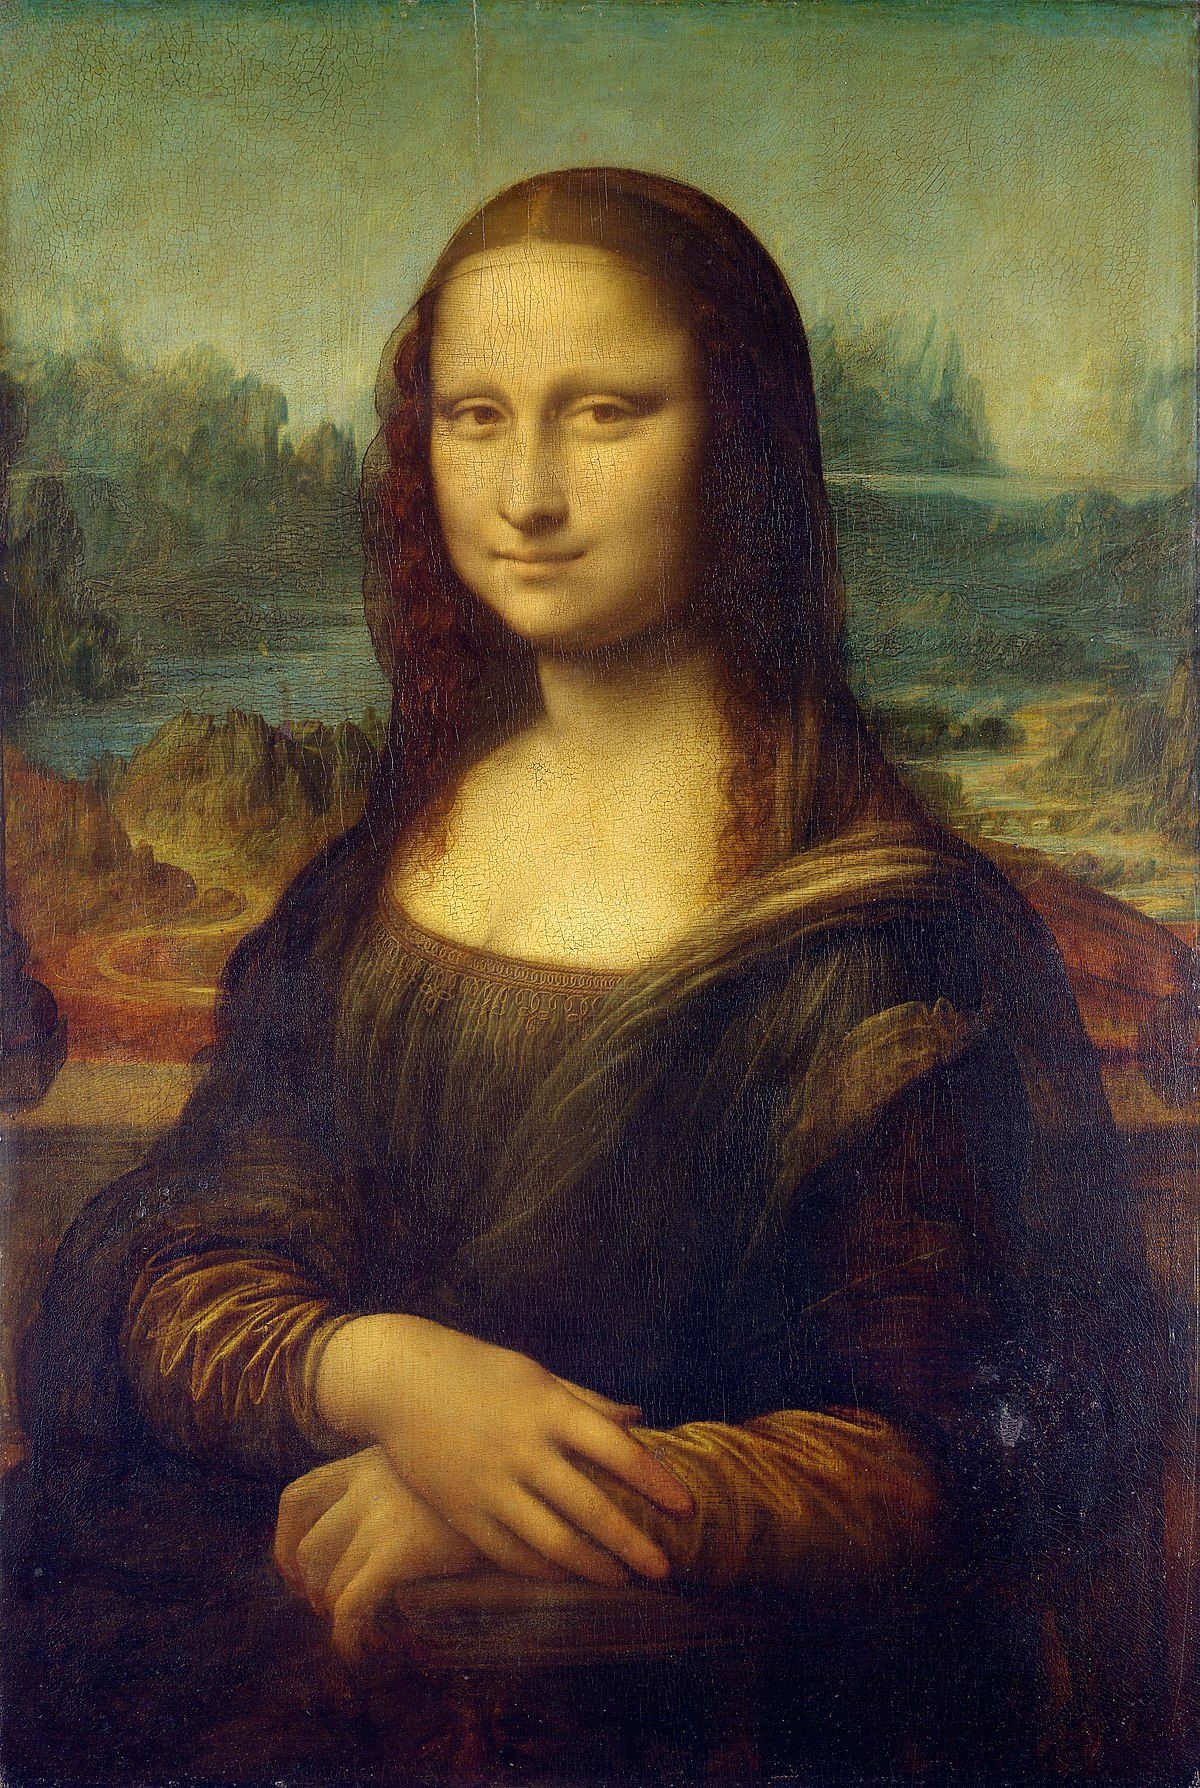
\includegraphics[width=.4\linewidth]{mona_lisa_original.jpg} }
    \subfloat{ 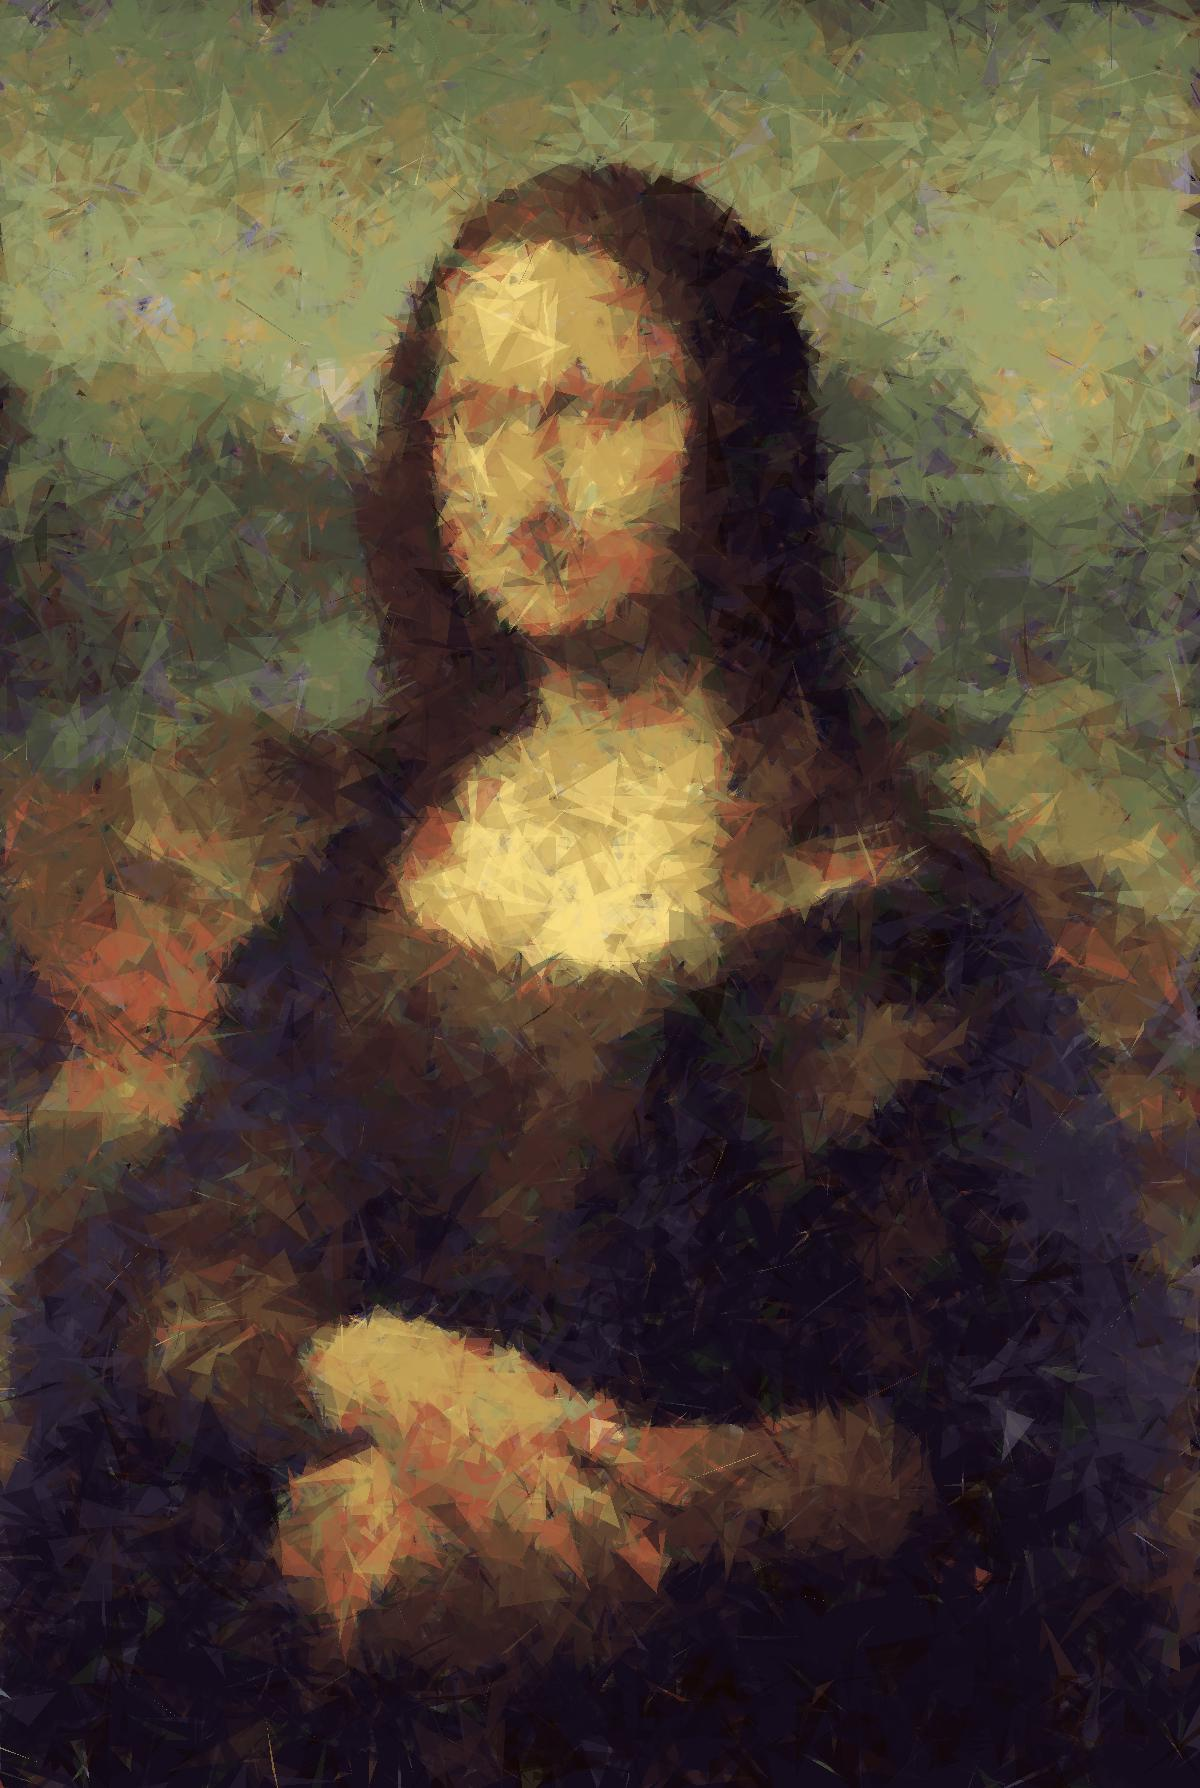
\includegraphics[width=.4\linewidth]{mona_lisa_candidate.jpg} }
    \caption*{Da Vinci, L. (1503-1519). Mona Lisa [Painting].}
    \label{fig:mona}
\end{figure}

\begin{CJK}{UTF8}{min}
\begin{figure}[H]
    \centering
    \subfloat{ 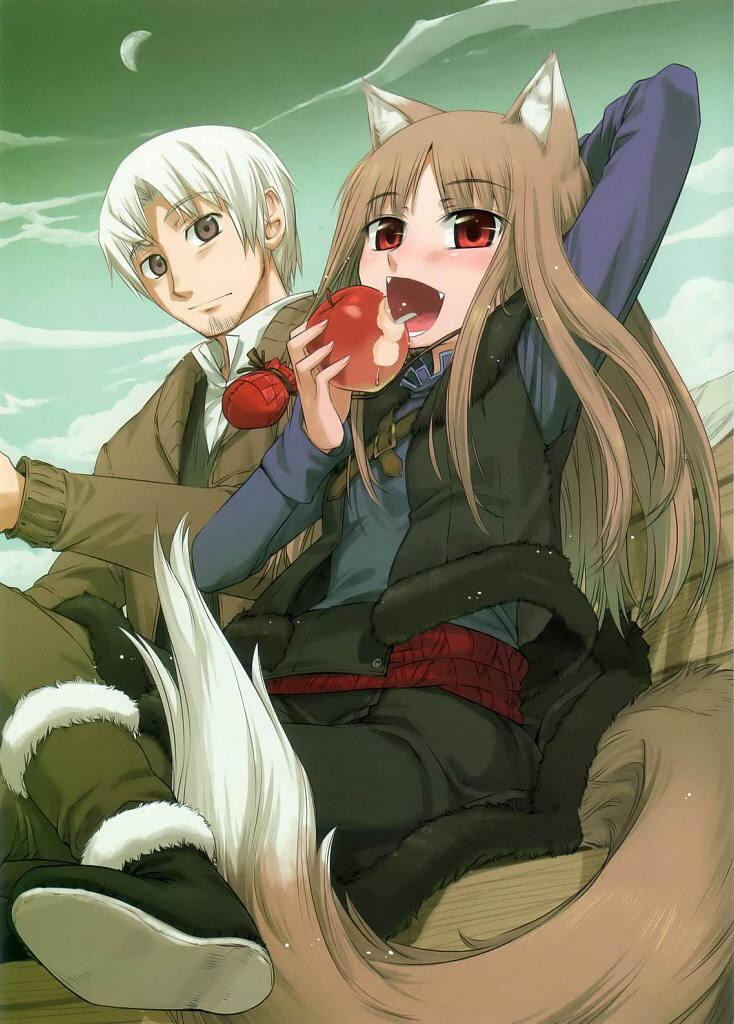
\includegraphics[width=.4\linewidth]{holo_original.jpg} }
    \subfloat{ 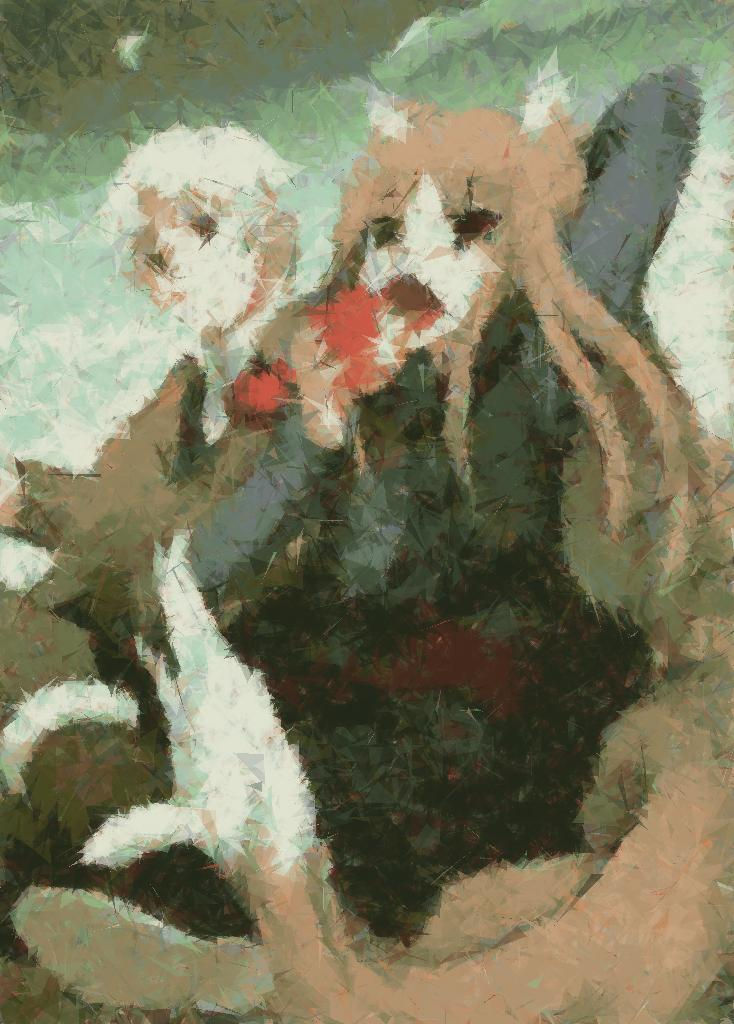
\includegraphics[width=.4\linewidth]{holo_candidate.jpg} }
    \caption*{文倉十 (Jū Ayakura). 狼と香辛料 (Ōkami to Kōshinryō) - Manga volume I cover (2008).}
    \label{fig:holo}
\end{figure}
\end{CJK}

\begin{figure}[H]
    \centering
    \subfloat{ 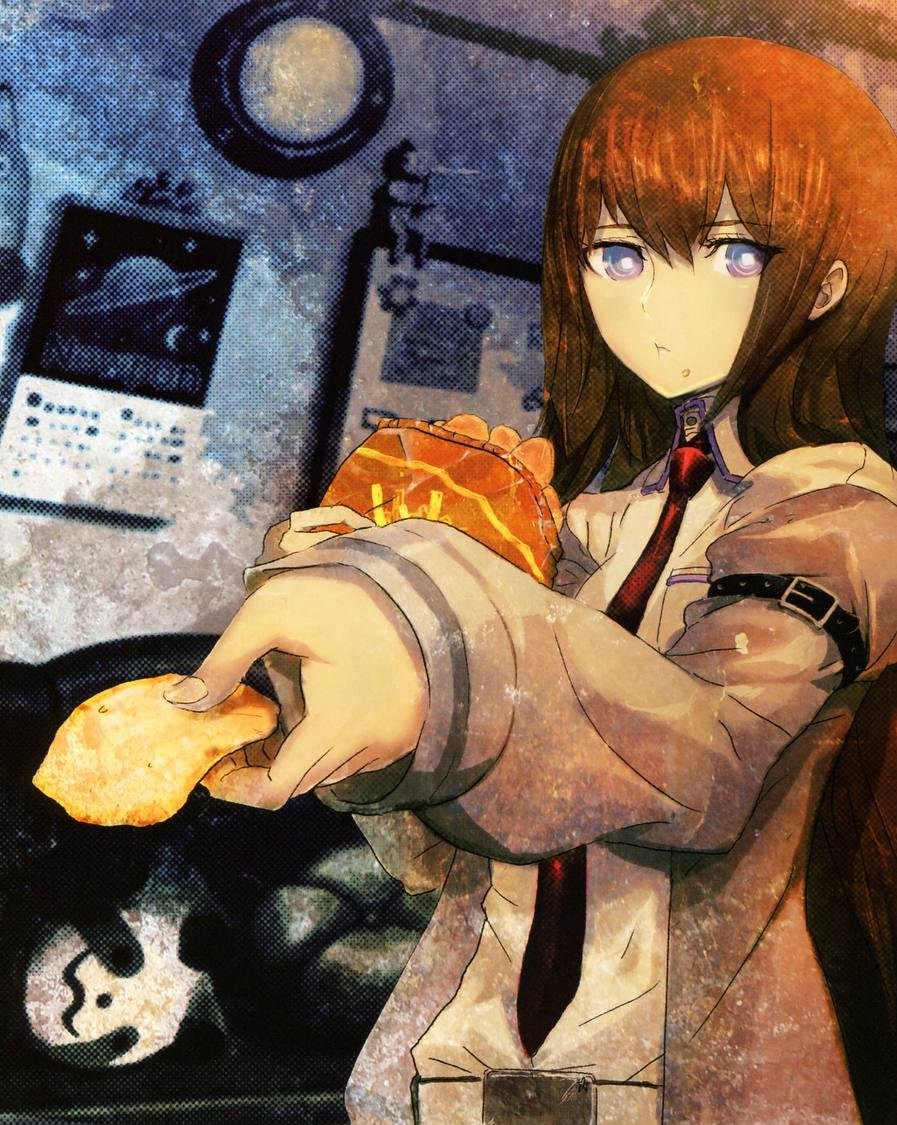
\includegraphics[width=.4\linewidth]{kurisu_original.jpg} }
    \subfloat{ 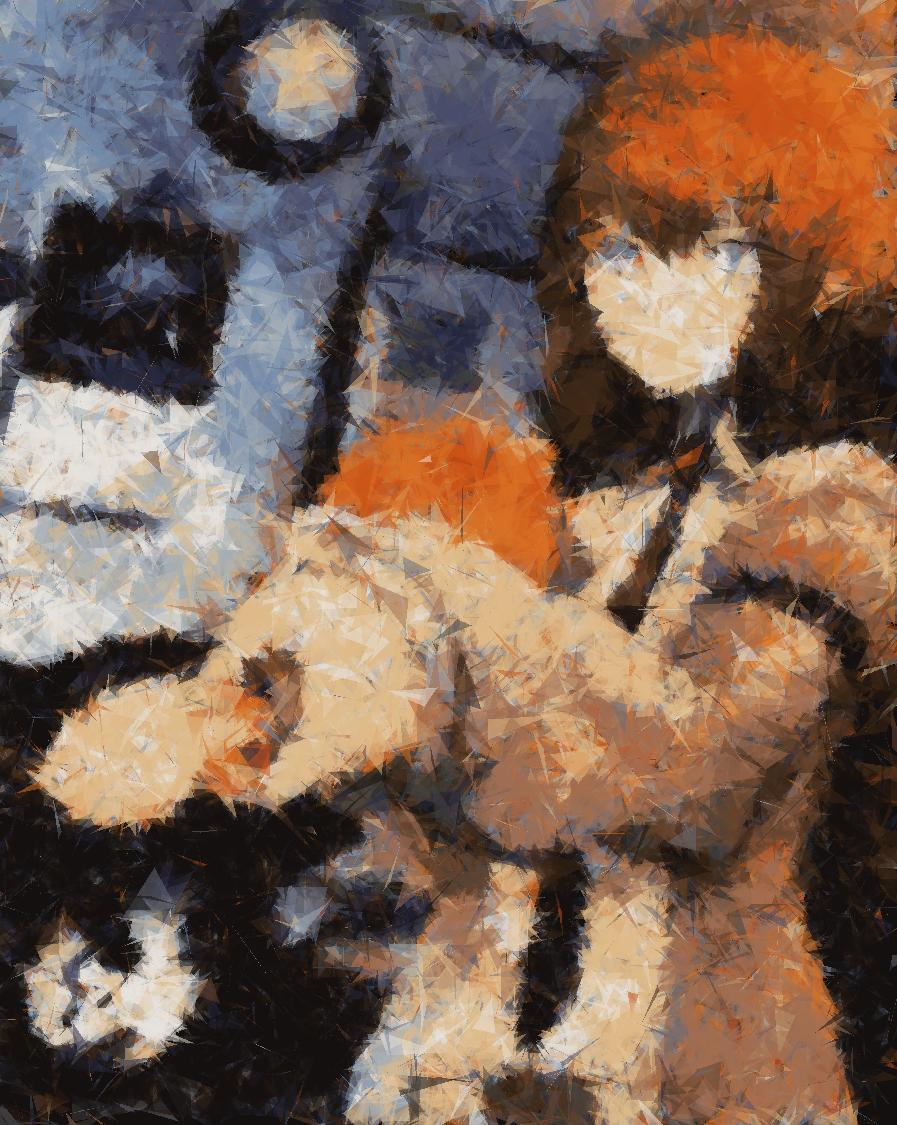
\includegraphics[width=.4\linewidth]{kurisu_candidate.jpg} }
    \caption*{Huke, (2013). Steins;gate Art Works imaginations of huke [Painting].}
    \label{fig:sailor}
\end{figure}

\begin{figure}[H]
    \centering
    \subfloat{ 
\includegraphics[width=.4\linewidth]{sailor_moon_original.jpg} }
    \subfloat{ 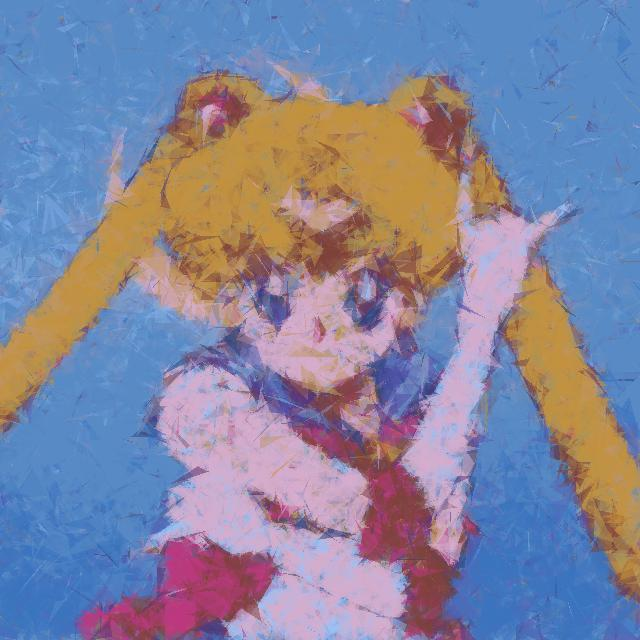
\includegraphics[width=.4\linewidth]{sailor_moon_candidate.jpg} }
    \caption*{Takeuchi et al., (1992-1997). Sailor Moon [TV series].}
    \label{fig:sailor}
\end{figure}

\begin{figure}[H]
    \centering
    \subfloat{ 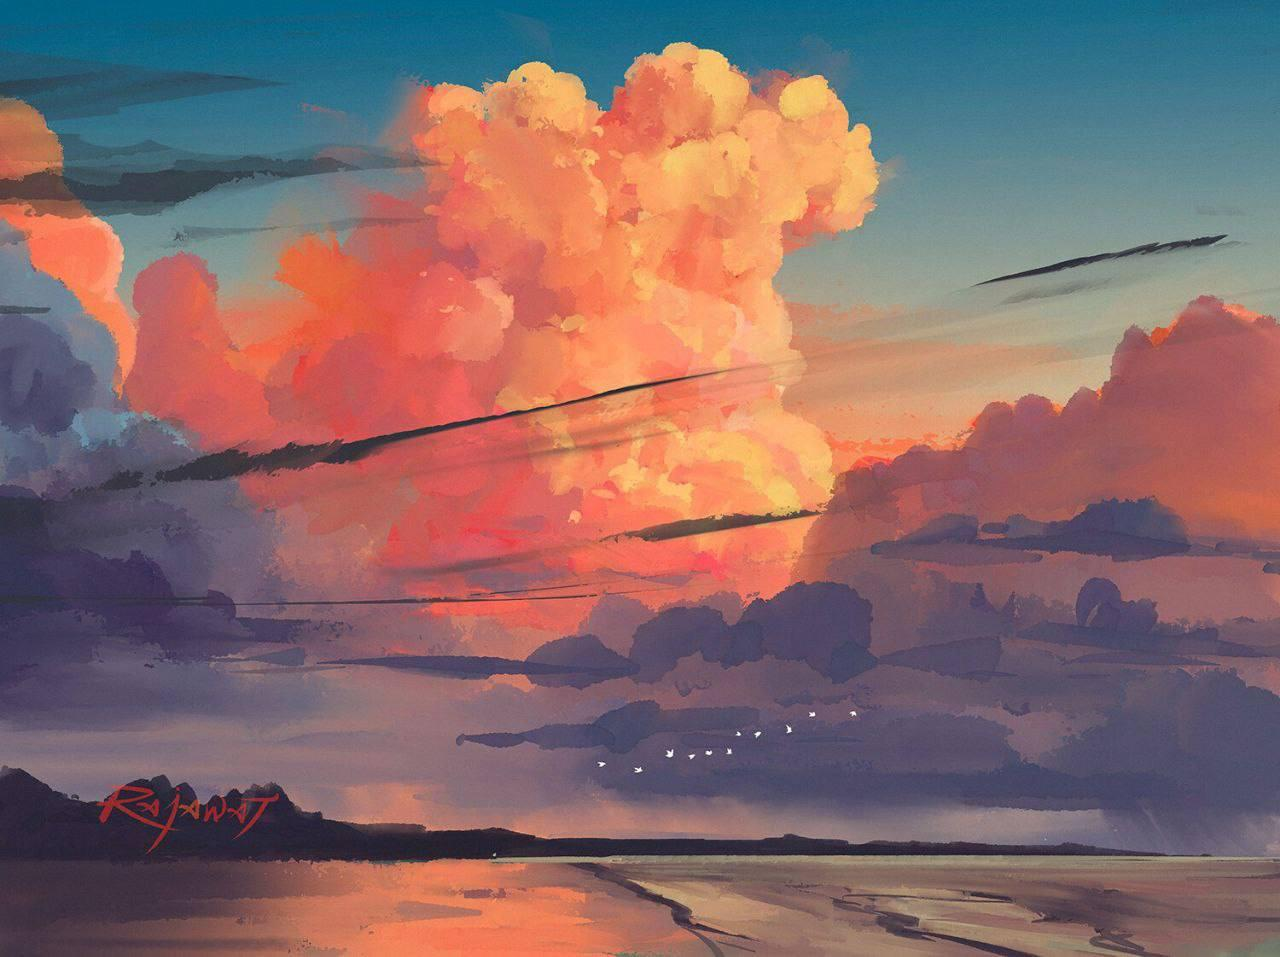
\includegraphics[width=.4\linewidth]{sunset_original.jpg} }
    \subfloat{ 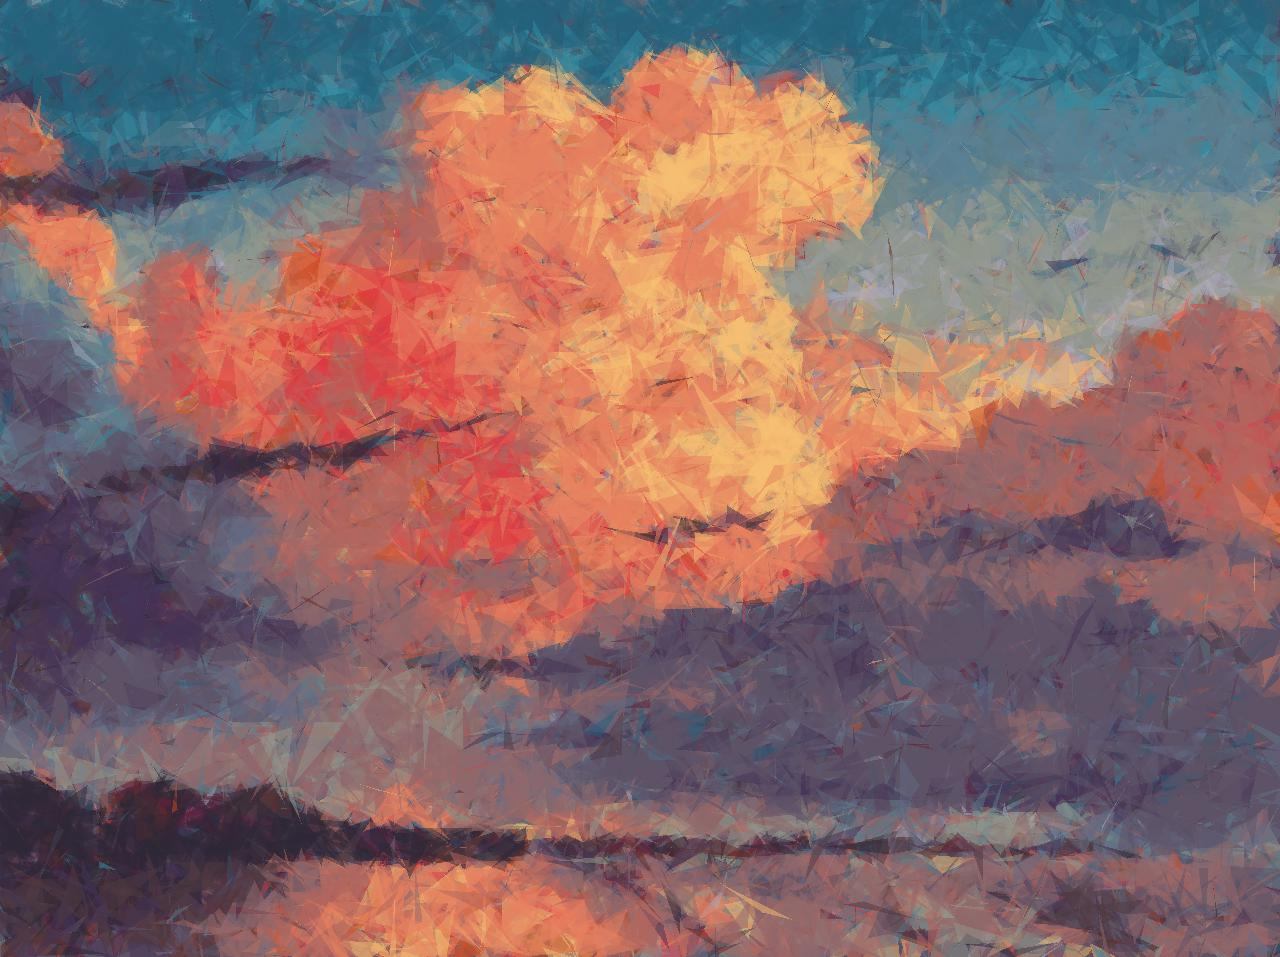
\includegraphics[width=.4\linewidth]{sunset_candidate.jpg} }
    \caption*{Rajawat, S. (2021). Daily Sketches [Painting].}
    \label{fig:sailor}
\end{figure}

\end{document}